\chapter{Baza danych}
Bazy danych pełnią kluczową rolę w strukturze wielu aplikacji, umożliwiając składowanie, organizację i efektywne zarządzanie danymi. Dzięki nim możliwe jest elastyczne dodawanie nowych informacji oraz rozwijanie funkcji systemu. Struktury baz danych są zoptymalizowane pod kątem efektywnego przeszukiwania i pobierania danych, co przyczynia się do wydajnego działania aplikacji. Dodatkowo, istnieje szereg narzędzi, takich jak \textbf{Spring Boot} i \textbf{Hibernate} (tabela \ref{tab:zestawienie_narzędzi}), które ułatwiają integrację z bazami danych, usprawniając tym samym proces ich obsługi.

\section{Model bazy danych}
\subsection{Opisy encji urządzeń}
W celu zdefiniowania struktury bazy danych stworzono diagram związków encji ERD (ang.~\emph{entity-relationship diagram}) jak na rysunku \ref{ErDiagram:label}.
\begin{figure}[b]
    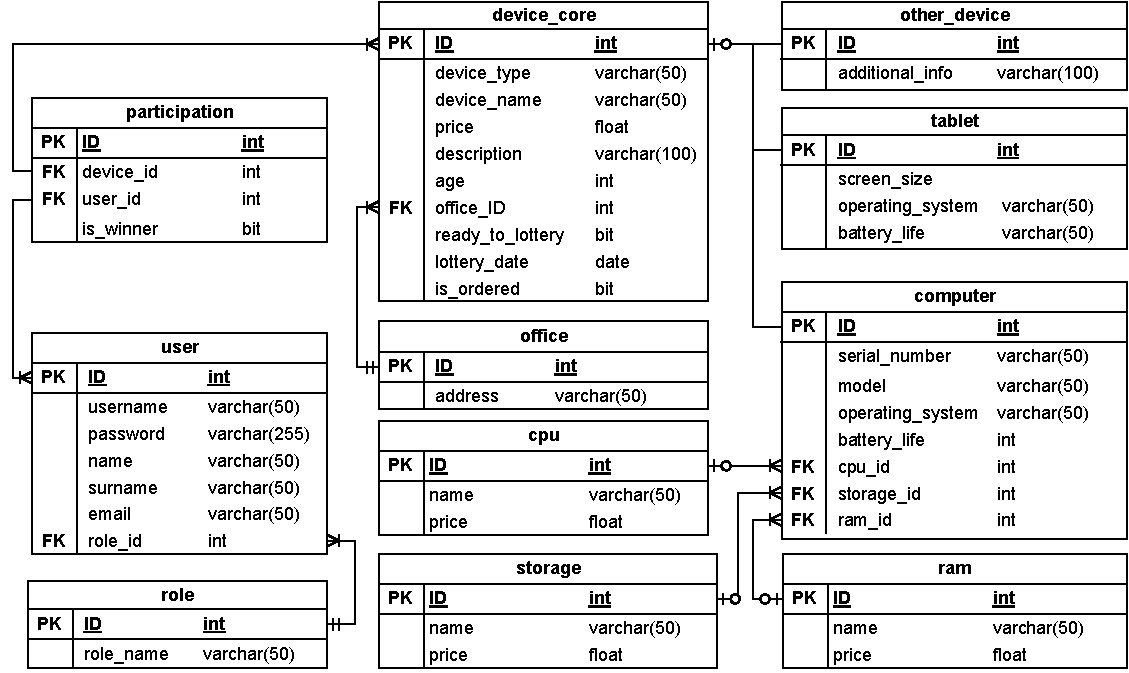
\includegraphics[width=\linewidth]{rys04/ER_Diagram.pdf}
    \caption{Diagram związków encji}
    \label{ErDiagram:label}
\end{figure}
Na diagramie tym zilustrowano, jakie typy danych są przechowywane w poszczególnych tabelach, a także jakie relacje zachodzą między tymi tabelami. Warto zaznaczyć, że ze względu na brak domyślnego wsparcia dla dziedziczenia tabel w relacyjnych bazach danych, zdecydowano się skorzystać z mechanizmu dziedziczenia dostępnego w Hibernate. Aspekt ten omówiono w dalszej części rozdziału.

W systemie istnieją różne rodzaje urządzeń, z których każdy jest reprezentowany przez odpowiadającą mu tabelę w bazie danych. Trzy główne kategorie urządzeń to: \texttt{computer}, \texttt{table} oraz \texttt{other\_device}. Wszystkie te kategorie dziedziczą swoje cechy od wspólnej tabeli o nazwie \texttt{device\_core}, która stanowi rdzeń dla wszystkich urządzeń.

Wspólny rdzeń, reprezentowany przez tabelę \texttt{device\_core}, zawiera parametry, które są dziedziczone przez wszystkie rodzaje urządzeń. Dzięki tej strukturze, każda tabela reprezentująca konkretny typ urządzenia posiada te same podstawowe atrybuty, ułatwiając jednolite zarządzanie nimi w systemie. Parametry wspólne dla wszystkich typów urządzeń obejmują: 
\begin{itemize}
	\item \texttt{ID} -- identyfikator urządzenia,
	\item \texttt{device\_type} -- typ urządzenia ułatwiający zarządzanie nimi w aplikacji klienckiej,
	\item \texttt{device\_name} --nazwa urządzenia,
	\item \texttt{price} -- cena urządzenia,
	\item \texttt{age} -- wiek urządzenia,
	\item \texttt{office\_id} -- identyfikator biura w którym znajduje się urządzenie,
	\item \texttt{ready\_to\_lottery} -- informacja czy sprzęt jest gotowy do przeprowadzenia loterii,
	\item \texttt{lottery\_date} -- data loterii w której odbyło się losowanie, jeżeli się nie odbyło to wartość jest pusta,
	\item \texttt{is\_ordered} -- informacja czy sprzęt został już odebrany przez pracownika.
\end{itemize}

Pozostałe tabele reprezentujące urządzenia rozszerzają informacje dostarczane przez rdzeń. Komputer dodatkowo posiada informacje odnośnie
\begin{itemize}
	\item \texttt{serial\_number} -- numer seryjny komputera,
	\item \texttt{model} -- model komputera,
	\item \texttt{operatinng\_system} -- system operacyjny zainstalowany na komputerze,
	\item \texttt{battery\_life} -- żywotność baterii,
	\item \texttt{cpu\_id} -- identyfikator reprezentujący procesor posiadany przez komputer,
	\item \texttt{storage\_id} -- identyfikator reprezentujący dysk posiadany przez komputer,
	\item \texttt{ram\_id } -- identyfikator reprezentujący pamięć RAM posiadaną przez komputer.
\end{itemize}


Tablet posiada dodatkowo informacje odnośnie:
\begin{itemize}
	\item \texttt{screen\_size} -- parametry wyświetlacza,
	\item \texttt{operatinng\_system} -- system operacyjny zainstalowany na tablecie,
	\item \texttt{battery\_life} -- żywotność baterii.
\end{itemize}
% TO DO: proszę zwrócić uwagę na listy wyliczeniowe (myślniki, przecinki, wielkość liter jak w listach powyżej)
% DONE
Inne urządzenie natomiast posiada tylko pole \texttt{additional\_info}, które pozwala na podanie szczególnych informacji urządzenia.

\subsection{Dziedziczenie tabel}
\label{dzedziczenie_hibernate:label}
Projektowany system powstał z myślą możliwości łatwego rozszerzania. Wykorzystanie tabeli \texttt{device\_core} ułatwi dodanie ewentualnych tabel potomnych. Kod tabeli nadrzędnej \texttt{device\_core} umożliwi wykonanie ogólnych operacji, co zapobiegnie powielaniu kodu oraz umożliwi dodanie tabel rozszerzających zakres danych zapisanych już w tabeli \texttt{device\_core}. 

Ważnym aspektem projektu jest zapewnienie unikalności kluczy w kontekście schematu dziedziczenia, szczególnie w przypadku użycia Hibernate z modelem \emph{TABLE\_PER\_CLASS}. W tym podejściu każda klasa dziedzicząca, tak jak \texttt{computer}, \texttt{tablet}, czy \texttt{other\_device}, ma swój własny identyfikator, ale także dziedziczy z klasy nadrzędnej. Hibernate programowo zarządza unikalnością kluczy dla całej hierarchii dziedziczenia, eliminując ryzyko konfliktów kluczy pomiędzy różnymi klasami. Dzieje się to na poziomie aplikacji. W praktyce, w bazie danych dla każdej klasy dziedziczącej, a także dla samej klasy \texttt{device\_core}, zostaną utworzone oddzielne tabele wykorzystując zapytania SQL generowane przez Hibernate. Tabele te zawierają wszystkie pola związane z daną klasą, a Hibernate zarządza relacjami między nimi. W przypadku klasy \texttt{device\_core}, tabela zawiera podstawowe atrybuty wspólne dla wszystkich typów urządzeń, takie jak \texttt{device\_name, price, age} itp. Przykład implementacji takiego dziedziczenia znajduje się w listingach kodu \ref{entity_deviceCore} i \ref{entity_computer}.
% TO DO: czy Hibernate robi to programowo (tj. jakimś specjalnym algorytmem)? Pytam, bo podobne rzeczy rozwiązuje się przez dołożenie do bazy danych triggerów
% DONE dodałem, że Hibernate programowo generuje zapytania SQL i zarządza identyfikatorami tabel 

Dla klas dziedziczących, takich jak \texttt{computer, tablet czy other\_device}, Hibernate generuje tabele z dodatkowymi kolumnami specyficznymi dla danej klasy, takimi jak \texttt{serial\_number} czy \texttt{screen\_size}. W efekcie każda tabela reprezentuje pełne zestawienie danych związanych z danym rodzajem urządzenia.



\section{Tworzenie bazy danych}
W tworzeniu baz danych istnieją dwa podejścia: \emph{code first} i \emph{database first}. W implementacji systemu wykorzystane zostało podejście \emph{database first}. Daje to w początkowym etapie projektowania większą przejrzystość danych. Po stworzeniu modelu można potem skorzystać z gotowych narzędzi, które pozwolą automatycznie wygenerować kod odzwierciedlający model danych.

Przy tworzeniu bazy danych wykorzystywanym narzędziem jest SSMS \ref{ssms:label}. Na początek stworzono tabele na podstawie diagramu związków encji \ref{ErDiagram:label} oraz określono jej relacje. Przykład tworzenia encji oraz jej relacji znajduje się na rysunku \ref{ssms_tworzenie:label}

\begin{figure}[htb]
  \centering
	\begin{tabular}{@{}ll@{}}
	a) & b) \\
  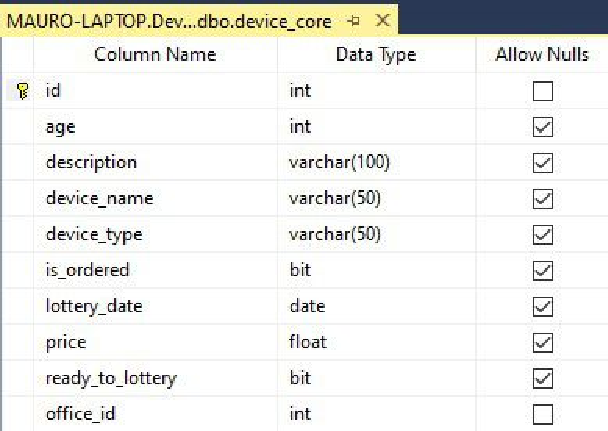
\includegraphics[width=0.445\textwidth]{rys04/design.pdf} & 
	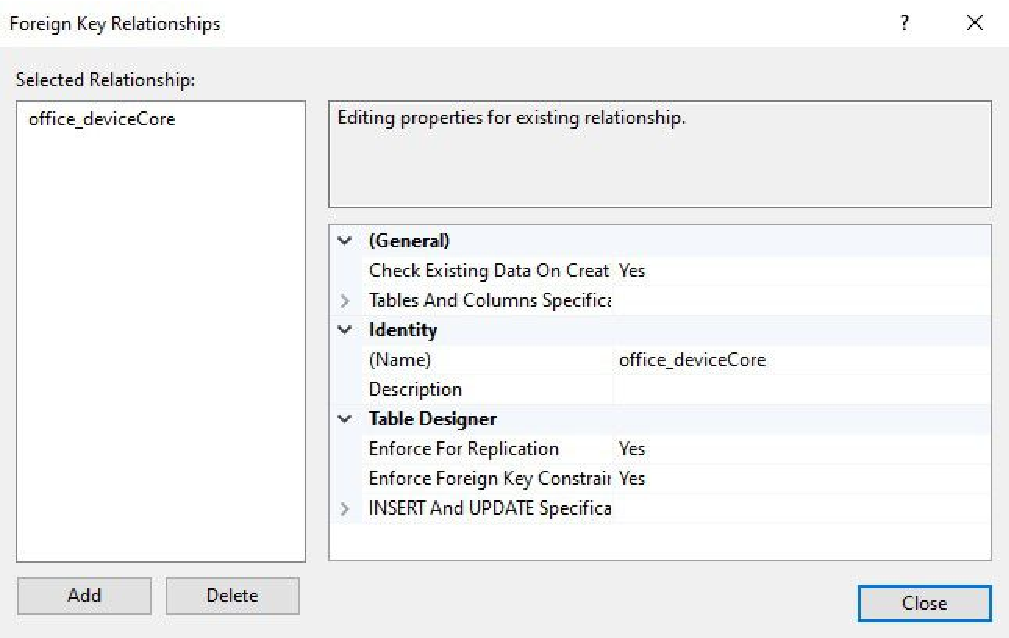
\includegraphics[width=0.505\textwidth]{rys04/relation.pdf}
	\end{tabular}
  \caption{Tworzenie bazy danych SSMS a) model, b) definiowanie relacji}
  \label{ssms_tworzenie:label}
\end{figure}

Po stworzeniu wszystkich tabel możliwe jest wygenerowanie kodu. Wykorzystano do tego plugin JPA Buddy oraz wbudowane narzędzia Intelij. Upraszcza to proces implementacji systemu. Na rysunku~\ref{generate:label} przedstawiono sposób generowania kodu encji dla klasy \texttt{computer}.
\makeatletter
\setlength{\@fptop}{0pt}
\makeatother
\begin{figure}[t!]
		\centering
    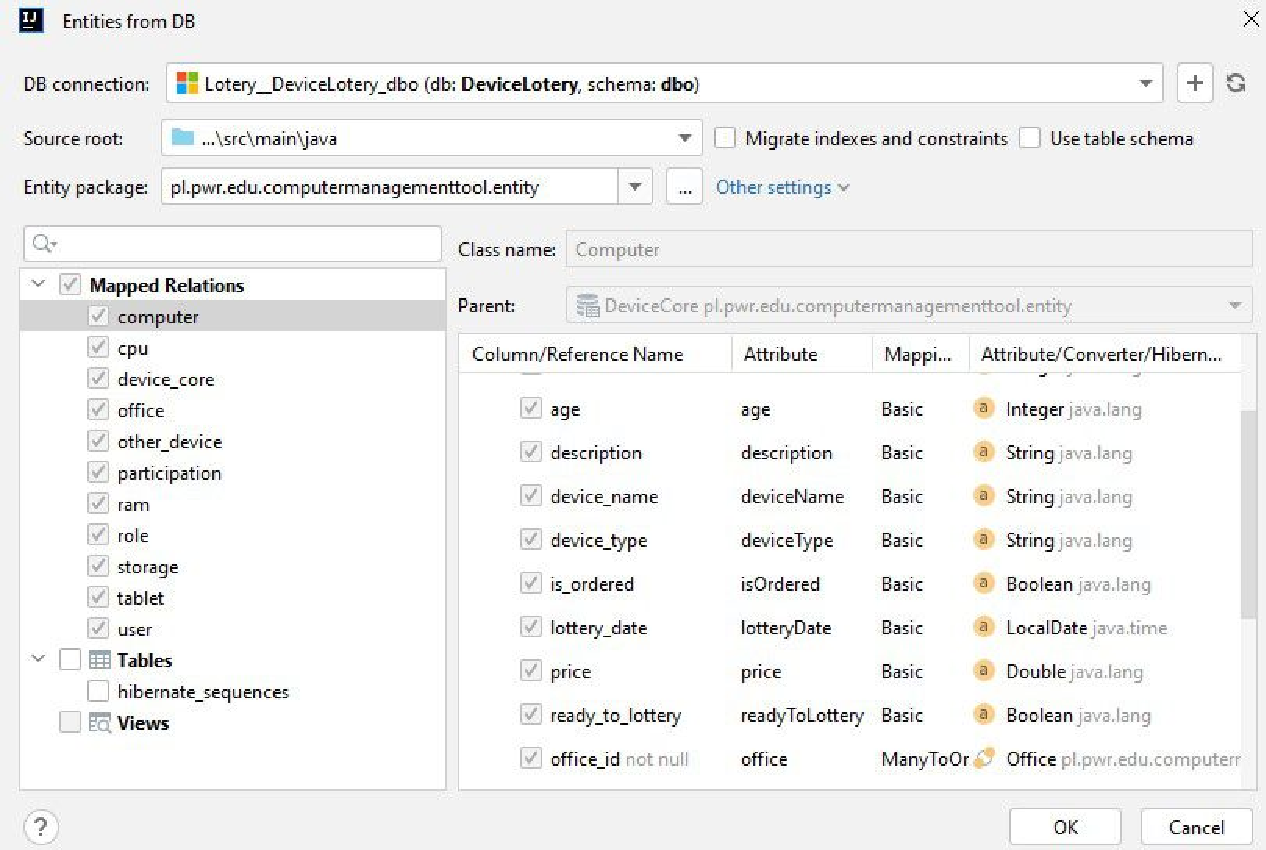
\includegraphics[width=0.7\linewidth]{rys04/generate.pdf}
    \caption{Generowaniu kodu na podstawie tabeli computer przy użyciu IntelliJ IDEA}
    \label{generate:label}
\end{figure}

Tworzenie w ten sposób początkowej struktury projektu jest bardzo pomocne. Jednak kiedy definiuje się sposób dziedziczenia tabel, to jedynym sposobem jest zdefiniowanie relacji wykorzystując Hibernate. O sposobie dziedziczenia tabel przez Hibernate napisano na początku tego rozdziału \ref{dzedziczenie_hibernate:label}. Szczegóły implementacji dotyczące klasy \texttt{device\_core} opisano w podrozdziale \ref{entity_deviceCore}. Odpowiednia konfiguracja projektu umożliwia aktualizowanie struktury bazy danych. Możliwe dzięki temu jest wyeliminowanie nadmiarowego kodu oraz skorzystanie abstrakcji dostarczanej przez dziedziczenie. Gdy Hibernate zaktualizuje strukturę bazy danych w SSMS automatycznie powstają odpowiednie tabele i relacje klas sprzętu. Zarządzanie unikalnością kluczy dla tych klas też jest możliwa tylko z poziomu kodu.
 
